% !TeX root = ../SPL-Challenges.tex
% !TeX spellcheck = en_US
\section{KICKin\textquotesingle \& Rollin\textquotesingle Challenge}

The objective of this challenge is for a robot to successfully kick a rolling ball from a ramp into a designated goal area. 
Each participating team will record three attempt sets, with a significant time between them.
A more specific schedule will be communicated closer to the competition.
An attempt sets consist of three kick attempts. 

\subsection{Field Setup}

\begin{figure}[t]
    \centerline{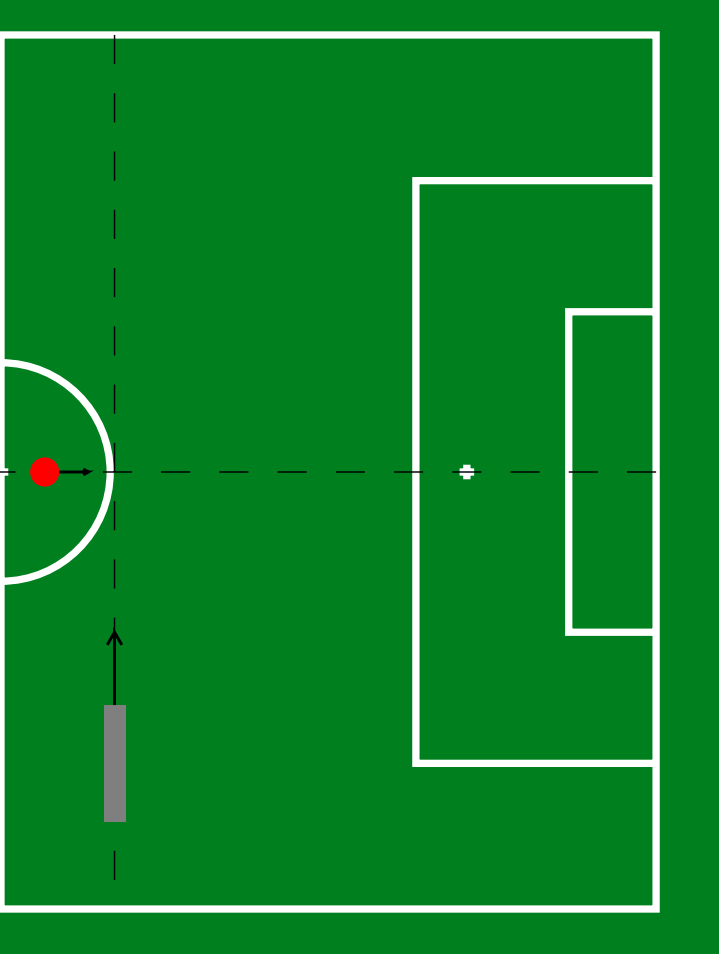
\includegraphics[width=\columnwidth/2]{figs/KICKin-Rollin-Placement-figure.png}}
    \caption{Illustration of robot and ramp placement for the challenge: The robot is depicted as a red dot, while the ramp is shown as a grey rectangle.}
    \label{fig:KICKin-Rolling-Challenge}
\end{figure}

The challenge will take place on a standard SPL field with its official marking. 
The ramp will be positioned perpendicularly adjacent to the halfway line, and aligned with a virtual line extending from the extremity of the center circle on the opponent's side.
The general idea is to position the Nao facing the goal, with the ball moving from its left to its right, or vice versa.
The ramp can be positioned at varying distances from the robots to modify the difficulty.
However, a minimum distance of 30 cm between the ramp and the virtual line must be maintained to ensure the ball rolls directly onto the field.
The participating robot can be positioned at the team’s discretion along the virtual line between the center circle and the penalty mark.
The robot must have one foot on each side of this virtual line.

\subsubsection{Ramp}

The selected ramp design will be made available on the SPL website. 
It may feature an adjustable angle to allow for modifications in difficulty.  

Teams are encouraged to propose their own ramp designs. 
For more information, visit the \url{https://spl.robocup.org/kickin-rollin-challenge-ramp/}.

\subsection{Challenge Procedure}

At the scheduled time, every participating must regroup on the designated field. 
The ramp will be set up by the technical committee and will remain the same for all attempts executed this day.
Each team will perform their three kicks successively.
Teams may bring as many robots as needed, but they will not be allowed to deploy code between attempts.

\subsection{Scoring}

Each kick will receive a score based on the location of the ball.
These points are non-cumulative: 

\begin{itemize}
	\item 0 points for a missed kick.
	\item 1 point for a deflected ball.
	A ball is considered deflected if it changes direction due to contact with the robot's feet.
	\item 2 points for kicking the ball.
	A ball is considered kicked if it makes contact with the front sensor of the robot's feet.
	\item 3 points for the ball entering the penalty area during the attempt. 
	If the ball leaves the area before coming to a complete stop, without qualifying for subsequent points, this still counts. 
	\item 5 points for the ball entering the goal. 
	\item 100 points for the ball going over the goal between the virtual planes of the two goalposts. 
  \end{itemize}

  A ball can only be considered kicked or deflected if it result from a direct action by the robot.
  Contact resulting from a stationary feet or a backward step will result in 0 points.

  \subsection{Ranking}

  Each team will be ranked based on the average of their best kick from each attempt.